\chapter{State of the Art in Virtual Commissioning} \label{sec:StateOfTheArt}
    In this chapter, the state of the art of virtual commissioning at PLC level is briefly listed and explained. For this purpose, the general procedure in a virtual commissioning is explained at the beginning and differences are compared. Then commonly used file formats for the required steps are shown.

\section{Foundations of Virtual Commissioning}
\subsection{Required Information for Virtual Commissioning}   \label{sec:DataForVirtualCommissioning}
    The development of a product includes several stages in different engineering disciplines as seen in \autoref{fig:StepsProductDevelopment}. These stages can partly be developed in parallel to save time and costs in the development process. However, special attention must be paid to the dependencies between the stages. \\
    
    The first phase of product development includes the general process of defining the objectives, constraints and interfaces. It is part of project management and must be worked out in close cooperation with the customer and possible suppliers. \\
    
    The next step is to develop the product's hardware usually consisting of mechanical and electrical components. The hardware must be developed in collaboration between both disciplines, since changes in the mechanics, for example, often also lead to changes in the electrics. This principle also applies in the opposite way. \\
    
    Parallel to the development of the hardware, the process of software development can be started already. In this way, possible limitations of the software can be identified at an early stage and possible changes to the finished hardware can be avoided. For the completion of the software, however, the hardware must already have been finalized. Only in this case testing and debugging is meaningful.  \\
    
    The final step in product development is an optional virtual commissioning followed by actual commissioning. Depending on the product, the start of series production or delivery to the customer takes place here. \\
    
    % oder https://tex.stackexchange.com/questions/320088/smartdiagram-package-different-fill-color-in-additionals
	\begin{figure}[htp]
        % Chevron Process
        \smartdiagramset{uniform sequence color=true,
            sequence item uniform color=gray!20,
            sequence item border color=white,
        }
	    \footnotesize
		\centering
		\begin{adjustbox}{width = \textwidth}
            \smartdiagram[sequence diagram]{Process Design, Mechanical Design, Electrical Design, PLC \\ Coding, (Virt.) Commissioning}
        \end{adjustbox}
		\caption{Steps in product development.}
		\label{fig:StepsProductDevelopment}
	\end{figure}
	
    Information from all phases of product development are required for the successful execution of a virtual or a real commissioning: 
    \begin{description}
        \item Process Design: Interfaces to other parts of the plant, such as transfer points of raw and finished parts, but also maximum time limits and throughput quantities. The selection and characteristics of used sensors and actuators also belong to this area. The characteristics of the used hardware is particularly important in the creation of behaviour models, where the information is given in data sheets or already integrated in models. 
        \item Mechanical Engineering: The general structure of the mechanics and the kinematics of the individual components are defined in this step. The design of the product and the used materials determine the physical behaviour and result in multiple CAD files. This information is often relevant for control systems. 
        \item Electrical Engineering: The configuration of the PLC with the used terminals is part of this section. Especially interesting for the development of the software is the mapping between the inputs and outputs of the terminals with the connected devices. Only an exactly documented mapping can avoid wrong connections in the PLC software and the resulting damage of the hardware. The documentation of the mapping and the structure of the PLC can be shown in a tabular form or in a dedicated object in the development environment of the PLC.
        \item PLC Coding: If more complex components are used in the plant, often these are addressed via their own interface. The documentation and the knowledge of handling these interfaces is important for the creation of the software but also for the later commissioning. In the best case examples exist, which explain the handling and therefore ensure a faster implementation. But also an example PLC code of simpler components can often be advantageous. 
    \end{description}



\subsection{Hardware or Software in the Loop (HIL/SIL)}
    In general, virtual commissioning at PLC level consists of two parts: the control system to be optimized and the simulation model that represents the real plant. The control itself is often tested on the real target hardware, but depending on the manufacturer, it can also be executed directly in the development environment on an engineering system. If the model instance is executed on a separate hardware, this is called \textit{hardware in the loop} (\acs{HIL}). In comparison, with \textit{software in the loop} (\acs{SIL}) the model instance is also executed on the target hardware. For a better understanding the setup of a HIL and a SIL system is shown in \autoref{fig:HIL_SIL}\\
    Depending on the complexity of the control system, both methods are suitable for the development and commissioning of PLC software. For example, basic functions and code sections can be tested quickly in a SIL system, thus shortening the development time. For more complex or time-critical controls, however, testing and commissioning is often easier to perform in a HIL system. \\
	\begin{figure}[htp]
		\centering
		\begin{subfigure}{.95\textwidth}
			\centering
			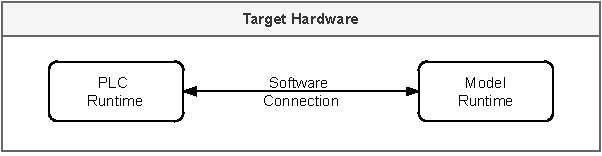
\includegraphics{figures/HilSilComparisonSIL.pdf}
			\caption{SIL system}
		\end{subfigure}
		\vspace{3mm}
		
		\begin{subfigure}{.95\textwidth}
			\centering
		    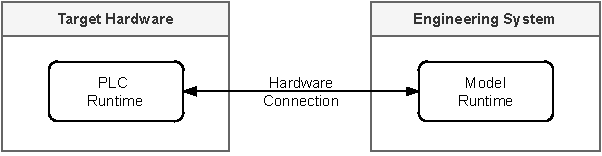
\includegraphics{figures/HilSilComparisonHIL.pdf}
			\caption{HIL system}
		\end{subfigure}
		\caption[Comparison of hardware setup in a SIL and HIL system.]{Comparison of hardware setup in a SIL and HIL system. While in a SIL system the model of the plant and the controller are executed on the same hardware, in a SIL system the model and the controller are executed on separate hardware.}
		\label{fig:HIL_SIL}
	\end{figure}
    
	The \ac{HIL} method offers advantages especially for complex systems compared to the \ac{SIL} method. The second hardware avoids performance problems due to the additional computations on the target hardware. Furthermore, this method is the better choice for automated testing, due to a simplified implementation of continuous regression testing. The goal of this type of testing is to detect errors and bugs due to newly created sections of code. The major drawback of this method is the additional communication between the controller and the model. This communication should be real-time capable to allow a meaningful simulation.\\
    One of the advantages of the \ac{SIL} method is the avoidance of additional hardware for the model instance in comparison with the \ac{HIL} method. Thus, in addition to the reduced cost of hardware, space in laboratories can also be saved. Finally, this results in a reduced planning effort for the laboratories and the time required for testing is shortened. One of the main requirements of the SIL system is the additional demand that the target hardware must be able to run the model of the plant in parallel with the control system.  \\
      
	
%\section{Different Approaches using Hard-/Software in the Loop}
    Testing and commissioning of the PLC software via HIL/SIL can be done in different ways, for which several practices are explained in the following lines. 

\subsubsection{Visualization in the PLC Development Environment}			% TwinCAT
	The \textit{human-machine interface} (\acs{HMI}) offers a quick possibility for testing the control software. In most cases, a graphical user interface can be created directly in the development environment in which current values and outputs of the control software can be displayed and inputs can be set. Depending on the used system this information can be processed even in or near to real-time. \\
	In this approach, the human developer imitates the behaviour of the real plant and therefore tries to identify potential problems in the software. Due to the human interaction, fast processes and reactions can only be tested to a limited extent. However, basic code sections and functions can be evaluated during development and in the process of a virtual commissioning. The creation of a \ac{HMI} is supported by many common PLC manufacturers such as \textit{Siemens} and \textit{Beckhoff}.
	
\subsubsection{Digital Twin using an Physics Engine}		% Unity		
    The next step in virtual commissioning is the use of an external physics engine such as \textit{Unity}. Especially by using existing libraries and well documented interfaces a simple model can be created in a short time. In addition, the handling of the model can be simplified by using the original geometry data. A disadvantage of this method compared to the direct visualization in the PLC development environment is the requirement of an additional communication between the PLC run-time and the physics engine. Nevertheless, depending on the implementation, this procedure can also be carried out in real-time. The area of application includes \ac{HIL} and also \ac{SIL} systems. By using the original CAD data, a visually appealing model can be created and controlled via the PLC. This is an important advantage especially in presentations with customers or in sales, in order to be able to address people from the non-technical area as well. But also the start for new employees in the development of the control is easier with a clear and appealing model. \\
    
    An example for the implementation in \textit{Unity} and \textit{TwinCAT} is \cite{DigitalTwinUnityExample}. Here, a digital twin is tested and used in a \ac{HIL} system, achieving a communication time of \SI{10}{\milli\second}. The simulation in \textit{Unity} achieves a step time of \SI{5}{\micro\second}.

\subsubsection{Digital Twin in a Simulation Software}		% Simulink
	The use of simulation software such as \textit{Matlab/Simulink} is particularly advantageous for complex systems or in control engineering. Complex systems can be easily created using mathematics and a graphical user interface. Furthermore, it improves the overview and minimizes the time needed to maintain the models. In this method, the model is executed in the simulation software and for this reason also requires additional communication to the PLC run-time. If the system is supposed to be real-time capable, special hardware or precautions are often required. This approach can also be used in \ac{HIL} and \ac{SIL} systems and is often found in final testing or the virtual commissioning of the software. 

\subsubsection{Visualization in a CAD Software}		% 
    The solution with probably the best overview is visualization directly in the CAD software. Through this possibility, a mechanical problem can be quickly identified and solved accordingly. The company \textit{Beckhoff}, for example, has recognized this opportunity and is currently developing its own product \textit{TE1130} with which the visualization can be done in a common CAD software. As said the product is still in development with the planned release date in end of 2022 \cite{BeckhoffCadProduct}. In any case, for each CAD tool used, a different interface depending on the manufacturer must be used to implement this possibility in practice. However, in this approach, only the visualization of the current state of the PLC is done in the CAD software and the model of the plant is not calculated.

\section{Relevant Data Formats}    \label{sec:AvailableDataFormats}
    This chapter describes and compares a selection of the most common data formats for relevant virtual commissioning information according to \autoref{sec:DataForVirtualCommissioning}.

\subsection{Geometry Data and Kinematization}		% step, COLLADA (kin)
% https://cadexchanger.com/formats/
	The branches of industry and their products are very diverse and with them the requirements for the used CAD software. For this reason, depending on the field of application, one specific CAD software may be more advantageous than another. Major CAD software vendors include \textit{Creo Elements}, \textit{Autodesk Inventor}, \textit{Solidworks} or \textit{Siemens NX}. \\ 
	A key feature in the design of components using CAD software is the handling with \textit{direct modeling} compared to \textit{parameterized modeling}. \\
	In \textit{direct} modeling, the geometry is generated using constant values. Through this static processing, the different elements of the geometry remain independent of each other and the model is simplified. This type of CAD software is mainly used in the static field, such as in structural engineering.  \\
	In contrast, in \textit{parameterized } modeling, the geometry is generated using dependencies and features. This results in a chronic listing of the steps that lead to the desired geometry. The individual components are then dynamically connected in an assembly, whereby geometric dependencies become visible. Due to this kinematization, the components can be easily moved in the software and attached components move with them. This is particularly advantageous in the dynamic area with moving parts for example in mechanical engineering.  \\
	
    The exchange of CAD data between different tools is usually done via neutral formats such as \textit{.step} (\acl{STEP}) or \textit{.iges} (\acl{IGES}). However, only the pure geometry is supported and transferred via these formats and an information loss of the kinematization and features occurs. If necessary, in this case the customer has to recreate the kinematization or the CAD exchange has to be done via native formats. In many areas and also in virtual commissioning, kinematization and thus its exchange is, however, an important prerequisite. The industry has recognized this problem of the missing interface of the kinematization and is therefore working on different solutions. \\
    For example, existing CAD data formats can be extended to support features and kinematization. For this purpose, this paper \cite{StepWithKin} proposes an possible extension of the \textit{.step} format in order to include the kinematization. However, this extension is not yet part of the standard and therefore not implemented in commercial CAD tools.  \\
    A second possibility is the development of a new and neutral data format, with the goal to be able to store the geometry and the kinematization. In order to be able to use this format, an integration into existing CAD tools can be implemented or, alternatively, a conversion of the native formats with the help of translators is also an option. However, both methods are feasible but require a major effort in technical and organizational terms. This paper \cite{PaperCADFeatureTranslator} shows the conversion of the native features in the design of a part into a neutral format and back into a second CAD software. The same approach could be used to export the kinematics as well as the features, as shown in this paper \cite{PaperCADConstrainTranslator}. \\
    As an alternative, the kinematics could be saved in an additional file and linked to the original CAD data. In this case, the CAD software would have to provide a way to save and read the kinematic separately from the assemblies. An example for this implementation is shown in this paper \cite{PaperConstrainWithStepAndXml}. Again, this method is feasible but requires a lot of effort, since a common agreement on the used data format has to be achieved and then implemented. \\
    A promising solution is the \textit{COLLADA} format (\acl{COLLADA}), which supports kinematization starting from version 1.5 \cite{ColladaSpecification}. The \textit{COLLADA} format, released back in 2004, is based on XML documents and is mainly used in the entertainment and gaming industry suffering from the same problem with a large number of incompatible tools. The use in the manufacturing industry is currently not attractive, because suitable tools for the conversion to and from native formats are still missing. However, the already widely used exchange format \textit{AutomationML} relies on the \textit{COLLADA} format to describe geometry data per default. 
    

\subsection{Behaviour Models}	% FMI https://fmi-standard.org/     -> Alternativen: Simpack, modellica, simulink, dymola, simulationx
    Similar to the geometry data, there is a variety of possible file formats for the description of a physical behaviour model. This is mostly dependent on the discipline and the simulation software used. For example, \textit{Simulink} and \textit{SimulationX} are available tools for describing physical systems in a wide range of possible application areas, whereby both tools use a native data format to describe a physical model. Alternatively, the \textit{Modelica} language can also be used for the description of a system as it is universal and offers the possibility to be integrated in a wide range of different tools.\\
    
    However, especially in the field of co-simulation a universal interface is required to simplify data exchange. This is needed due to the combination of multiple engineering disciplines and tools for a complete simulation of the device under test. For this reason, the \ac{FMI} was defined by \textit{Modelica Association} already in 2010 and is currently in fact the default format for exchanging models. The basis of this interface consists of C-code, which can be used universally on different devices. Currently this interface is available in version 3 and is already supported by more than 170 different tools \cite{FmiSpecification}. This great popularity is also the result of the publicly available tools for checking the compatibility of \textit{FMI} objects save as \ac{.fmu} files and a open source distribution of the sources. 

\subsection{Source Code of PLC Projects}		% PLCopen
    In the area of control engineering and automation using PLCs, the basis is mainly the international IEC~61131 standard. In the context of this thesis, Part 3, which defines the programming languages, is of particular interest. 
    This standard is based to a large extent on the organization \textit{PLCopen}, which has set itself the goal of increasing the efficiency in the creation of control software and to be platform-independent between different development environments. To make this possible the PLC project with its code and libraries are saved as \textit{XML} files and therefore can be exchanged without problems. This exchange format was standardized in 2019 in Part 10 of the IEC~61131 standard. \\
    
    Many PLC manufacturers rely on this standard and offer interfaces for the defined programming languages. As a result, the effort required to exchange the software and thus the costs can be minimized. 


\subsection{Documentation}		% PDF, MD, HTML
	Only good documentation ensures the proper use of a product. This should be easy to read and understand by humans, thereby avoiding incorrect handling. For this purpose, various file formats are available, such as: \textit{.pdf} (\acl{PDF}), \textit{.md} (\acl{MD}) or \textit{.html} (\acl{HTML}). The individual file formats all offer advantages and disadvantages, whereby the selection of the suitable format depends thereby strongly on the intended use. \\
	
    For example, a \textit{.pdf} file offers high compatibility between different devices combined with easy handling. 
    The \textit{.md} format is mainly used by software developers due to its standard integration with Git and easy handling. Formatting texts is very easy and the integration of lists, images and tables is possible. 
    In web-based help pages the \textit{.html} format is often used. It can be displayed in any browser and is therefore, similar to the \textit{.pdf} format, independent of the platform. \\
    
	In any case, the use of plain text files for more complex documentation should be avoided. The missing possibility to embed images and to link between sections and files results in a documentation that is difficult to understand. However, simple instructions are excluded from this. 

\subsection{Exchange Libraries}     % AutomationML
    When data is exchanged between supplier and customer via different tools, there should ideally be no loss of information. This goal cannot always be achieved, but using existing and especially supported exchange formats like \textit{AutomationML} increases the probability of success.  \\
    This format represents thereby different information such as hierarchy, schematics and also code. By default, an object is composed in \textit{AutomationML} from the geometry as \textit{COLLADA} file and the control code in \textit{PLCopen} format. Additional information can be added as desired as in the case of behaviour models as \ac{FMI} files. This approach is for example seen in \cite{AutomationMLWithFMU}. For this reason, \textit{AutomationML} represents an appropriate exchange format \cite{PaperIsAMLanAppropriateExchangeFormat}. However, as mentioned above, the lack of support for the \textit{COLLADA} format from the CAD software side is still a problem.
    
    


%\section{Version Control}
\section{Criteria for a Data Structure in Virtual Commissioning} \label{subsec:CriterionsForDataStructure}
    Based on these fundamentals of a virtual commissioning, criteria for a data structure can be identified. With the help of these criteria, the efficiency of a data structure can be determined, whereby these should be fulfilled as good as possible. The identified criteria are: 
 %   To effectively use a data structure in a virtual commissioning, the following criteria must be fulfilled:
    \begin{itemize}
        \item Independent of used hardware setup (HIL/SIL).
        \item Contain all needed information.
        \item Modular layout in order to represent components of a real plants.
        \item High compatibility with common software tools (Data formats).
        \item Low level of additional knowledge required / Easy to use.
    \end{itemize}


\section{Summary} 
    This chapter describes the current state of the art in the field of virtual commissioning of a PLC. With that in mind, the basics of virtual commissioning, consisting of the physical structure and the required information, are described at the beginning. This information results from all stages of product development and are available in various data formats. \\
    In the second part, relevant data formats for the identified information are described. These data formats include: CAD, behaviour model, source code of the PLC, documentation and existing exchange formats. Based on these conclusions, the development of a data structure for a modular virtual commissioning is done. \\
    Finally, criteria are defined by which a data structure for virtual commissioning may be evaluated.
  
  % Von Product development  
%    This chapter provides an overview of the individual steps in the development of a product. This process begins with basic project management with the specification of requirements and interfaces. After that, the hardware consisting of mechanics and electrics is developed and then the software is written. The final step is commissioning. \\
 %   The second part of this chapter covers the information required for virtual commissioning. It should be remembered that information from all steps of product development are required.
  
  